%=========================================================================
% (c) 2014, 2015 Josef Lusticky

\chapter{40 Gigabit Ethernet}\label{chap:40gbe}
The 40 and 100~Gigabit Ethernet were ratified in 2010 as the IEEE 802.3ba standard~\cite{ieee-802.3ba}.
These speeds open doors to significantly higher-capacity networks
and enable networks to scale in ways that were previously impossible.
The 40 and 100~GbE operate in full duplex mode only.
This is also the first time two speeds have been included in an Ethernet standard.

A rough estimate of the CPU processing required to handle a given Ethernet link speed is that
one hertz of CPU processing is required to send or receive one bit.
This general rule of thumb was first stated by PC Magazine in the mid 1990's,
and it is still used as a rule of thumb today~\cite{10gea-toe}.

The core networking doubles its speed approximately every 18 months, whereas
CPU I/O performance doubles every 24 months.
The growth of Ethernet speed has already surpassed
the growth of microprocessor performance~\cite{10gea-toe}.
Figure~\ref{fig:40gbe-performance-gap} shows,
that the 802.3ba Ethernet standard further extends the performance gap.
\begin{figure}
	\centering
	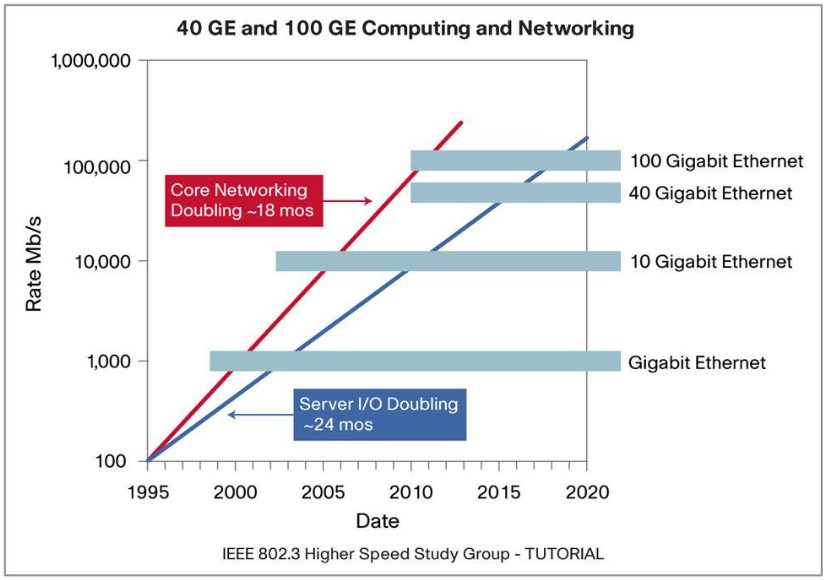
\includegraphics[width=13cm,keepaspectratio]{fig/performance-gap.png}
	\caption{Network and CPU performance gap (source:~\cite{cisco-market-need})}
	\label{fig:40gbe-performance-gap}
	\bigskip
\end{figure}

The 802.3ba standard specifies the physical coding sublayer that is common to both
40 and 100~Gb/s physical layer implementations~\cite{ieee-802.3ba}.
This physical coding sublayer is known as 40GBASE-R and 100GBASE-R.
802.3ba further specifies the following 40~GbE port types.
All of them use 4 fiber pairs and 40GBASE-R physical coding.
\begin{itemize}
\item 40GBASE-SR4 runs over multimode fiber with Short reach for at least 100~m range
\item 40GBASE-LR4 runs over single mode fiber with Long reach, with the required operating range at least 10~km
\item 40GBASE-CR4 is a Copper type over twinaxial cable
\item 40GBASE-KR4 is a port type for bacKplanes
\item 40GBASE-ER4 with an Extended operating range at least 30~km, which
is currently under discussion by the IEEE P802.3bm 40GBASE-ER4 Task Force~\cite{ieee-802.3bm}.
\end{itemize}

The 40GBASE-SR4 runs on Quad (4-channel) Small Form Factor Pluggable (abbreviated as QSPF or QSPF+).
QSPF is a high-density fiber connector with 12 strands of fiber.
Each channel has a dedicated transmit fiber and a dedicated receive fiber.
The middle four fibers remain unused~\cite{cisco-market-need}.
The channel layout is shown in figure~\ref{fig:40gbe-ethernet-layout}.
\begin{figure}
	\centering
	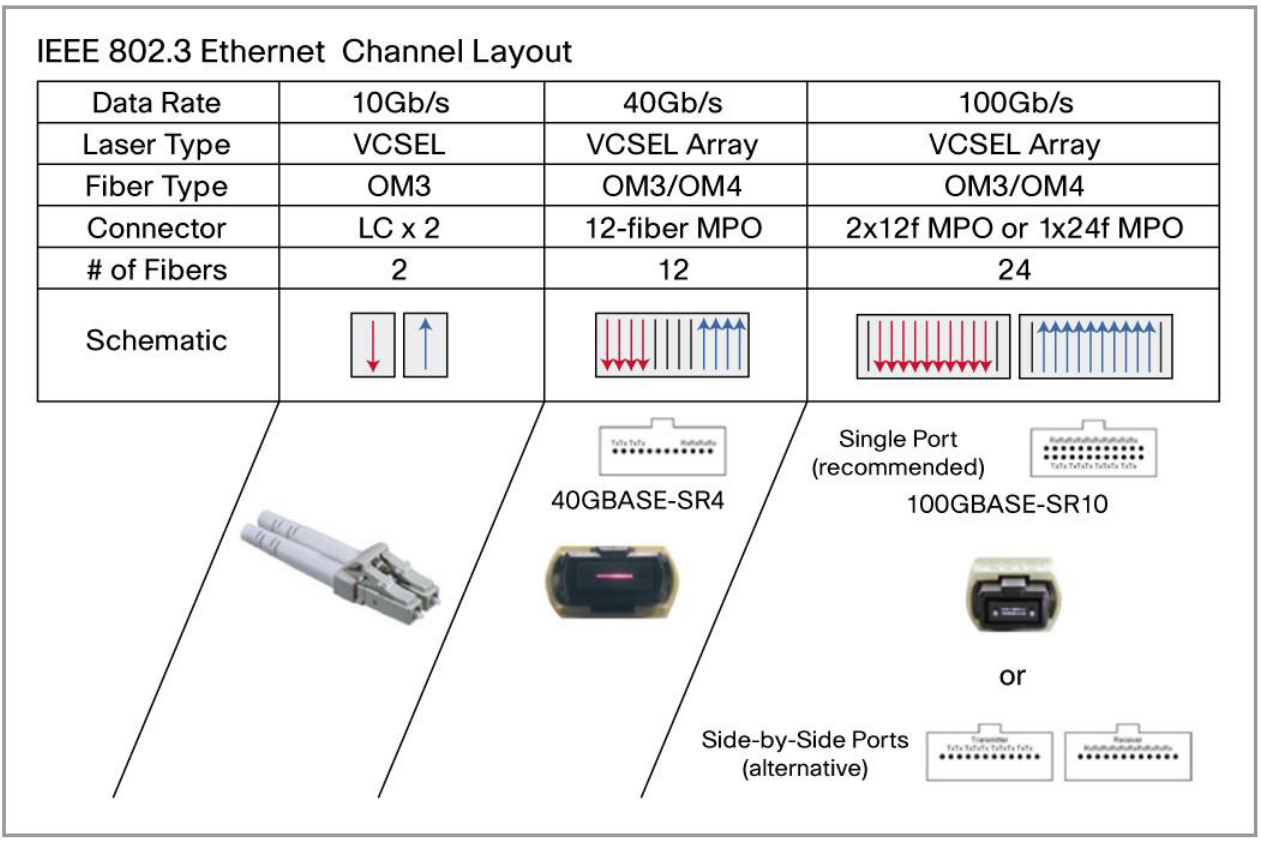
\includegraphics[width=13cm,keepaspectratio]{fig/ethernet-layout.png}
	\caption{IEEE 802.3 Ethernet Channel Layout (source:~\cite{cisco-market-need})}
	\label{fig:40gbe-ethernet-layout}
	\bigskip
\end{figure}

%=========================================================================
% (c) 2014, 2015 Josef Lusticky

\section{Frame rates}\label{sec:40gbe-frame-rates}
At 40 Gigabits per second rate, it takes $\frac{8}{40 \times 10^{9}} = 0.2~ns$ to transfer a single octet.
The time to transfer a whole frame depends on its size.
The standard Ethernet frame size remains unchanged in the IEEE 802.3ba standard and
is between 72 and 1526~octets.
Frames are separated by the Interframe gap (IFG) - a pause between two consecutive frames.
In 40 and 100~Gigabit Ethernet,
the length of IFG may vary due to clock tolerance and lane alignment requirements,
but it must be at least 1 octet.
The mean length of IFG is 12~octets~\cite{ieee-802.3ba}.

Figure~\ref{fig:40gbe-ethernet-frame} shows the Ethernet frame format with no extensions (e.g. 802.1Q VLAN tag).
Each frame starts with an 8-octet Preamble, which consists of a 7-octet pattern of alternating 1 and 0 bits,
and 1 octet of 1010~1011 value called Start of Frame Delimiter~(SFD).
The SFD is designed to break the previous 7-octet pattern and to signal the start of the actual frame~\cite{ieee-802.3ba}.

The Destination MAC address, Source MAC address and Type or Length fields form the link-layer Ethernet header.
The Type or Length field represents Type in case of Ethernet II (DIX) frame
and Length in case of IEEE 802.3 frame.
Both formats are in use today~\cite{understanding-internals}.

The Payload field represents the transferred Layer~3 data of a variable size.
The size of the data is bound by the standard Ethernet frame size and can be up to 1500~octets,
which is the Maximum Transmission Unit (MTU) of Ethernet~\cite{ieee-802.3ba}.
Frame Check Sequence (FCS) is a 4-octet cyclic redundancy code to check the integrity of the received frame.

\begin{figure}
	\centering
	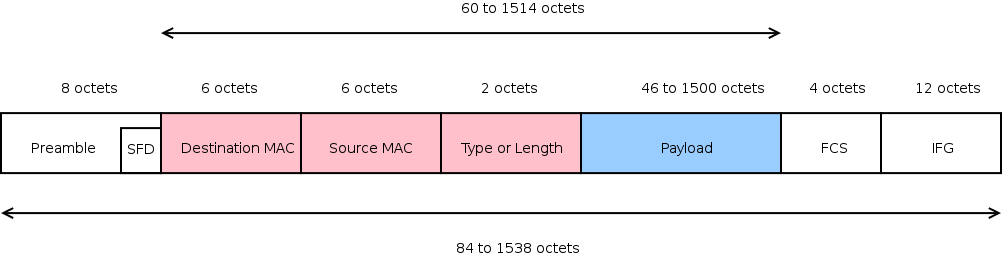
\includegraphics[width=15cm,keepaspectratio]{fig/ethernet-frame.png}
	\caption{Ethernet frame format}
	\label{fig:40gbe-ethernet-frame}
	\bigskip
\end{figure}

The Preamble, FCS and IFG carry no data and provide a necessary overhead of 24~octets for each frame.
The size of this overhead is independent from the Payload size.
Upon arrival of a frame, the rest is transferred from a network adapter to the host CPU and processed.
The data in the Ethernet header (Source and Destination MAC addresses and Type or Length) are used for L2 processing.
The data in the Payload field are used for L3 processing (i.e. routing).

The maximum sized frame is 1538 octets including the Interframe gap
(8-octet Preamble + 14-octet Ethernet header + 1500-octet Payload + 4-octet FCS + 12-octet Interframe gap).
At 40~Gbps rate, a traffic consisting of only the maximum sized frames of 1538 octets
produces $\frac{40 \times 10^{9}}{1538 \times 8} = 3~250~975$ frames per second.
In reference to the minimum frame size of 84~octets including IFG,
the 40~Gigabit Ethernet can transmit up to $\frac{40 \times 10^{9}}{84 \times 8} = 59~523~809$~frames per second.

Since each frame must be processed separately,
such high frame rates require enormous fast processing speed.
Despite the continual frame rates increases,
the 1500 byte Maximum Transmission Unit (MTU) of Ethernet remains unchanged.

Extensions to allow larger frames were made by several vendors.
The typical maximum sized jumbo frames in use are 9~038 octets (carrying 9~000 octets of Payload)~\cite{ea-jumbo-frames}.
The 40~GbE transmits $\frac{40 \times 10^{9}}{9038 \times 8} = 555~555$~of such jumbo frames per second at full rate.


%=========================================================================
% (c) 2014, 2015 Josef Lusticky

\section{Throughput}\label{sec:40gbe-throughput}
With 40~GbE, not only the per frame processing became a concern.
In case of the maximum sized frames,
40~Gbps Ethernet NIC transfers $3~259~452 \times 1514 \doteq 4.6$~GB/s of L2 data
(Ethernet header and Payload) to the host CPU.
Since the frame overhead is independent from its size,
the efficiency of Ethernet drops significantly with smaller frames.
In case of the minimum sized frames, the transfer rate drops to $59~523~809 \times 60 \doteq 2.6$~GB/s
while still operating at 40~Gbps rate.
Such data rates require appropriate bus between the NIC and the CPU to operate at full speed.

A single PCI-Express 2.0 lane provides throughput of 5~Gigatransfers per second in each direction~\cite{pcie-specification}.
In this case, Gigatransfer per second is the same as gigabit per second,
but it also includes the bits that are lost as a result of the interface overhead.
PCI-Express 2.0 uses 8b/10b coding, that is, 8 bits of data cost 10 bits to transfer (the same as in SATA case)~\cite{pcie-bandwidth}.
Therefore, the actual bandwidth is 500~MB/s per lane.
A PCI-Express 2.0 link with 8 lanes provides 4~GB/s throughput,
which is not enough to transfer the 40~GbE traffic between the NIC and the CPU.
The widest 16-lanes link doubles the throughput to 8~GB/s, which is sufficient for a 40~GbE adapter.

PCI-Express 3.0 increases throughput to 8~Gigatransfers/s in each direction for a single lane~\cite{pcie-specification}.
Additionally, it uses more efficient 128b/130b coding.
This way, a bandwidth of 984.6~MB/s per lane is achieved, almost twice the PCI-Express 2.0.
An 8-lane PCI-Express 3.0 link provides 7~876.8~MB/s bandwidth which is sufficient to handle 40~GbE traffic.

The above calculations do not include an additional overhead of the PCI-Express link headers
and signalling interrupts.
The PCI-Express devices are required to support the Message Signalled Interrupts (MSI) feature~\cite{pcie-specification}.
MSI is a technique to generate interrupts by writing to a specified address,
which has been written into the peripheral's configuration during initialisation.
The interrupt signalling consists of sending a Write request over the PCI-Express link
to the specified address~\cite{pcie-tutorial-1}.
There can be up to 32 MSI interrupts assigned to a single device,
but the number of interrupts the device uses must be a power of 2~\cite{msi-driver-guide}.

MSI-X is an extension to the MSI mechanism, which introduces various new features.
MSI-X provides support for signalling an interrupt directly to a particular CPU
and it allows to use up to 2048 interrupts and the number of interrupts is not restricted to a power of 2.
This feature is used by modern 40~GbE adapters to spread
the work related to traffic processing among multiple CPUs.
The device can use either MSI or MSI-X, but not both simultaneously~\cite{msi-driver-guide}.

Although both PCI-Express 2.0 x16 and PCI-Express 3.0 x8 links can be used for 40~GbE cards,
NIC vendors tend to produce 40~GbE PCI 3.0 x8 adapters,
because a PCI-Express x8 adapter can be plugged into a x16 slot, but not the other way round~\cite{pcie-specification}.
An adapter with less lanes saves both costs and troubles finding an empty x16 slot.


%=========================================================================
% (c) 2014, 2015 Josef Lusticky

\section{Compatibility}\label{sec:40gbe-compatibility}
The previous 10~Gigabit Ethernet standard was ratified by the IEEE 802.3 Working Group in 2002~\cite{ieee-802.3ae}.
As opposed to 40~GbE, the cabling plant of 10~GbE uses just a single pair of fiber.
In 2013, Cisco introduced a replacement that does not require a change to the cabling plant
and makes it possible to run 40~GbE over a single pair of multimode fiber~\cite{40gbe-mmf}.

Since its ratification in 2002,
it took four years to standardise 10~GbE over copper twisted pair 10GBASE-T in 2006~\cite{ieee-802.3an}.
10GBASE-T can run over a Category~6 cable within the range of 55m.
For full 100m range, a Category~6a cable is required~\cite{ieee-802.3an}.
One of the previous barriers to 10GBASE-T adoption was the power consumption per port compared to other 10 GbE options.
However, improvements in semiconductor manufacturing technology
significantly decreased power use to the point where it is no longer a concern.
Nowadays, 10GBASE-T and Category~6A cabling costs less than optical fiber technology~\cite{belden-10g-40g}.

The 40~GbE over Category~8 copper twisted pair
is currently being discussed by the IEEE P802.3bq 40GBASE-T Task Force.
The maximum range for 40GBASE-T is planned to be just 30 meters~\cite{ieee-802.3bq}.
Such range should be sufficient for most switch-to-server connections in data centres.
Because of the shorter distance, the power consumption of 40GBASE-T should be less than of 10GBASE-T~\cite{belden-10g-40g}.

40~Gigabit Ethernet is backward compatible with its predecessor.
Due to concerns around vendor and equipment interoperability,
IEEE has determined they will not support or define Jumbo frames~\cite{ea-jumbo-frames}.
Modern 100Mbps or higher Ethernet also uses constant signalling, which avoids the need for the preamble~\cite{anatomy-frame}.
However, the frame format is preserved for today's Ethernet transmission speeds to avoid making any changes.
With the upcoming 40GBASE-T variant, 10M/100M/1G/10G/40G link speed auto-negotiation can be expected in the future.

The 40~Gigabit Ethernet protocol support was introduced in the Linux kernel by various NIC vendors.
Red Hat Enterprise Linux 7 supports 40 Gigabit network interface controllers since its initial release~\cite{rhel-7-announce}.
Additional support was also introduced in RHEL 6.6~\cite{rhel-66-announce}.

